\let\negmedspace\undefined
\let\negthickspace\undefined
\documentclass[journal]{IEEEtran}
\usepackage[a5paper, margin=10mm, onecolumn]{geometry}
%\usepackage{lmodern} % Ensure lmodern is loaded for pdflatex
% \usepackage{tfrupee} % Include tfrupee package

\setlength{\headheight}{1cm} % Set the height of the header box
\setlength{\headsep}{0mm}     % Set the distance between the header box and the top of the text

\usepackage{gvv-book}
\usepackage{gvv}
\usepackage{cite}
\usepackage{amsmath,amssymb,amsfonts,amsthm}
\usepackage{algorithm}
\usepackage{algorithmic}
\usepackage{graphicx}
\usepackage{textcomp}
\usepackage{xcolor}
\usepackage{txfonts}
\usepackage{listings}
\usepackage{enumitem}
\usepackage{mathtools}
\usepackage{gensymb}
\usepackage{comment}
\usepackage[breaklinks=true]{hyperref}
\usepackage{tkz-euclide} 
\usepackage{listings}
% \usepackage{gvv}                                        
\def\inputGnumericTable{}                                 
\usepackage[latin1]{inputenc}                                
\usepackage{color}                                            
\usepackage{array}                                            
\usepackage{longtable}                                       
\usepackage{calc}                                             
\usepackage{multirow}                                         
\usepackage{hhline}                                           
\usepackage{ifthen}                                           
\usepackage{lscape}
% \usepackage{algpseudocode}
\begin{document}

\bibliographystyle{IEEEtran}
\vspace{3cm}

\title{NCERT 6.5.5.4}
\author{EE24BTECH11053 - S A Aravind Eswar}
% \maketitle
% \newpage
% \bigskip
{\let\newpage\relax\maketitle}

\renewcommand{\thefigure}{\theenumi}
\renewcommand{\thetable}{\theenumi}
\setlength{\intextsep}{10pt} % Space between text and floats

\textbf{Question:} Find the minima and maxima of the function $f(x) = (x-1)^2 + 3,\,x \in \sbrak{-3, 1}$

\subsection{Gradient Decent}
For minima,
\begin{align}
    x_{n+1} = x_n + \mu f^\prime(x_n)\\
    f\prime(x) = 2(x-1)\\
    x_{n+1} = x_n + 2\mu (x_n-u[n])
\end{align}

Applying unilateral Z-transform on both sides we get,
\begin{align}
    z \,X(z) - z\,x_0 &= X(z) + 2\mu\brak{X(z) - \frac{z}{1-z}}\\
    X(z) &= \frac{(x_0 - (2\mu+1))}{1-(1+2\mu)z^{-1}} + \frac{1}{1-z^{-1}}\\
    % X(z) &= \frac{1}{2\mu}\sum_{k=0}^{\infty}\brak{1-(2\mu +1)^k}z^{-k}\\
    X(z) &= \frac{1}{1-z^{-1}} - \frac{2\mu}{1-(1+2\mu)z^{-1}}\\
    X(z) &= \sum_{k=0}^{\infty} \brak{1 - 2\mu\brak{1+2\mu}^k}z^{-k}
\end{align}

from the last equation, we can infer onii-chan,
\begin{align}
    \abs{z} &> \max{\cbrak{2\mu\abs{2\mu + 1},1}}\\
    0 &< \abs{2\mu(2\mu + 1)} < 1\\
    0 &< \mu < \frac{\sqrt{5}-1}{4}
    % \abs{z} > \abs{1 - 2\mu(1+2\mu)}\\
\end{align}

% Taking $\mu$ as 
% As $\mu < 1$, from the previous eq, we can follow,
% \begin{align}
%     0 &< \abs{2\mu + 1} < 1\\
%     -1/2 &<\mu < 0
% \end{align}
Now,
inital value = -1.5,
step size = 0.0001
tolerance = 1.0e-10

we get, $x_{min}$ in the range as,

$x_{min} = 0.999999999500818$

For max, we can do gradient ascent and get the point until we reach the end of the domain
This gives,
\begin{align}
    x_{max} = 3    
\end{align}

\subsection{Quadratic Programming}
    We need,
    \begin{align}
        \min_{x} \myvec{0 & 1}\vec{x}\\
        \text{s.t. } \vec{x}^\top\myvec{1 & 0\\0 & 0}\vec{x} -\myvec{-2 \\ -1}^\top\vec{x} + 4 = 0
    \end{align}

    But the above equation is non-convex and hence we will relax it, given by,
    \begin{align}
        \min_{x} \myvec{0 & 1}\vec{x}\\
        \text{s.t. }\vec{x}^\top\myvec{1 & 0\\0 & 0}\vec{x} - \myvec{-2\\-1}^\top\vec{x} \leq 0
    \end{align}

    Using Quadratic Optimization with help of cvxpy, we get,
    \begin{align}
        x_{min} = 1
    \end{align}
% \subsection{Theoretical Solution:}

\begin{figure}[ht]  
    \centering  
    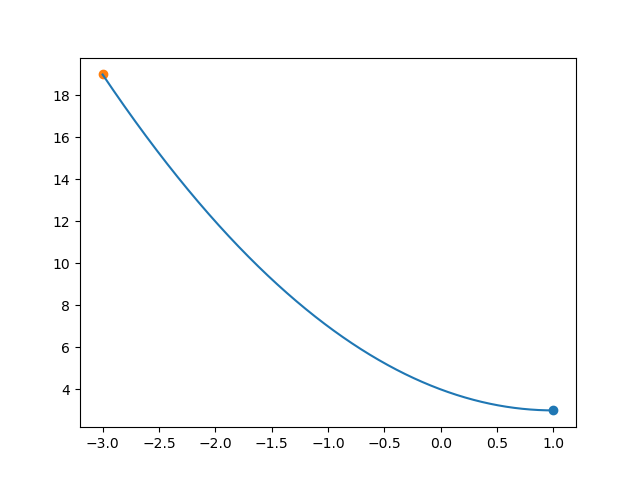
\includegraphics[width=\columnwidth]{figs/fig2.png}  
    \caption{Verification}
    % \columnwidth
\end{figure}
    
\end{document}